%!TEX root = ../../../../memoria.tex
\section{\themesCPT}

	La aplicación permite cambiar el \themeCPT fácilmente.
	Una de las partes más importantes del \frameworkPC \ecommerceCOM corresponde justamente a la customización de la aplicación, dado que esto logra generar identidad. A modo de ejemplo, se mostrarán importaciones de \themesCPT en el \frameworkPC. Para esto se utilizará los \themesCPT gratuitos que proporciona \bootswatchNAME. Esta tarea es muy sencilla, y basta con agregar el \refsource{source:less:generic_bootswatch_theme} al final del archivo generado por \bootstrapPackage llamado \textbf{custom.reaction.import.less}.

	\medskip
	\begin{lstlisting}[caption= Código genérico para importar \themesCPT desde \bootswatchNAME., label=source:less:generic_bootswatch_theme]
		@import "http://bootswatch.com/THEME-NAME/bootswatch.less";
		@import "http://bootswatch.com/THEME-NAME/variables.less";
	\end{lstlisting}

	En donde \textbf{THEME-NAME} corresponde a algún \themeCPT de los disponibles en el sitio de \bootswatchNAME. En particular, los \themesCPT \textbf{\themeUnited}, \textbf{\themeJournal}, \textbf{\themeCerulean}, \textbf{\themeSuperHero}, \textbf{\themePaper}, \textbf{\themeSimplex} y \textbf{\themeYeti} se pueden apreciar en las Figuras \ref{figure:bootstrap:theme_united}, \ref{figure:bootstrap:theme_journal}, \ref{figure:bootstrap:theme_cerulean}, \ref{figure:bootstrap:theme_superhero}, \ref{figure:bootstrap:theme_paper}, \ref{figure:bootstrap:theme_simplex} y \ref{figure:bootstrap:theme_yeti}, respectivamente.


	\begin{figure}[H]
		\centering
		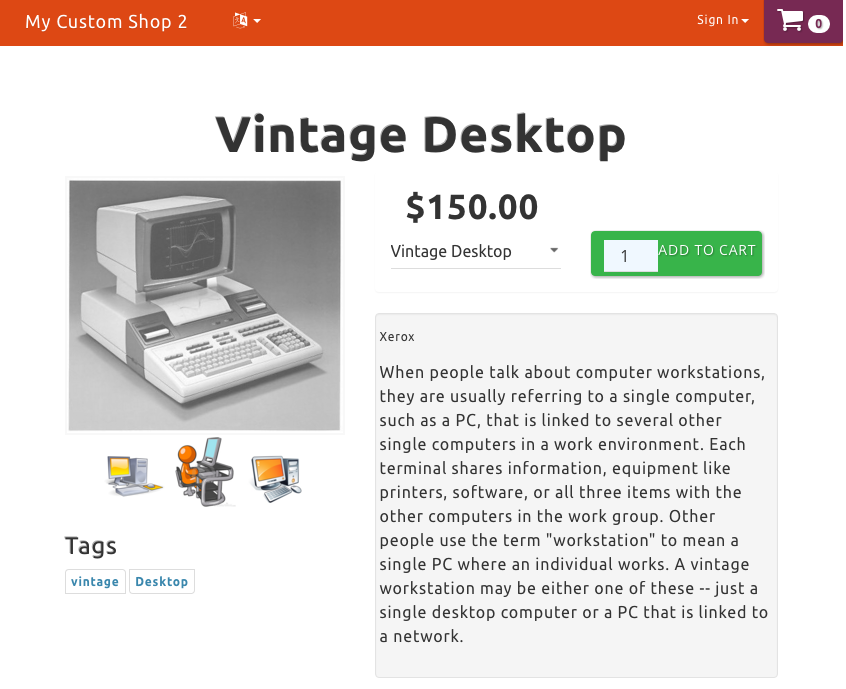
\includegraphics[width=0.6\textwidth]{figuras/bootstrap/bootstrap_theme_united.png}

		\caption{Descripción de un producto utilizando el \themeCPT \textbf{\themeUnited} del sitio \bootswatchNAME.}
		\label{figure:bootstrap:theme_united}
	\end{figure}

	\begin{figure}[H]
		\centering
		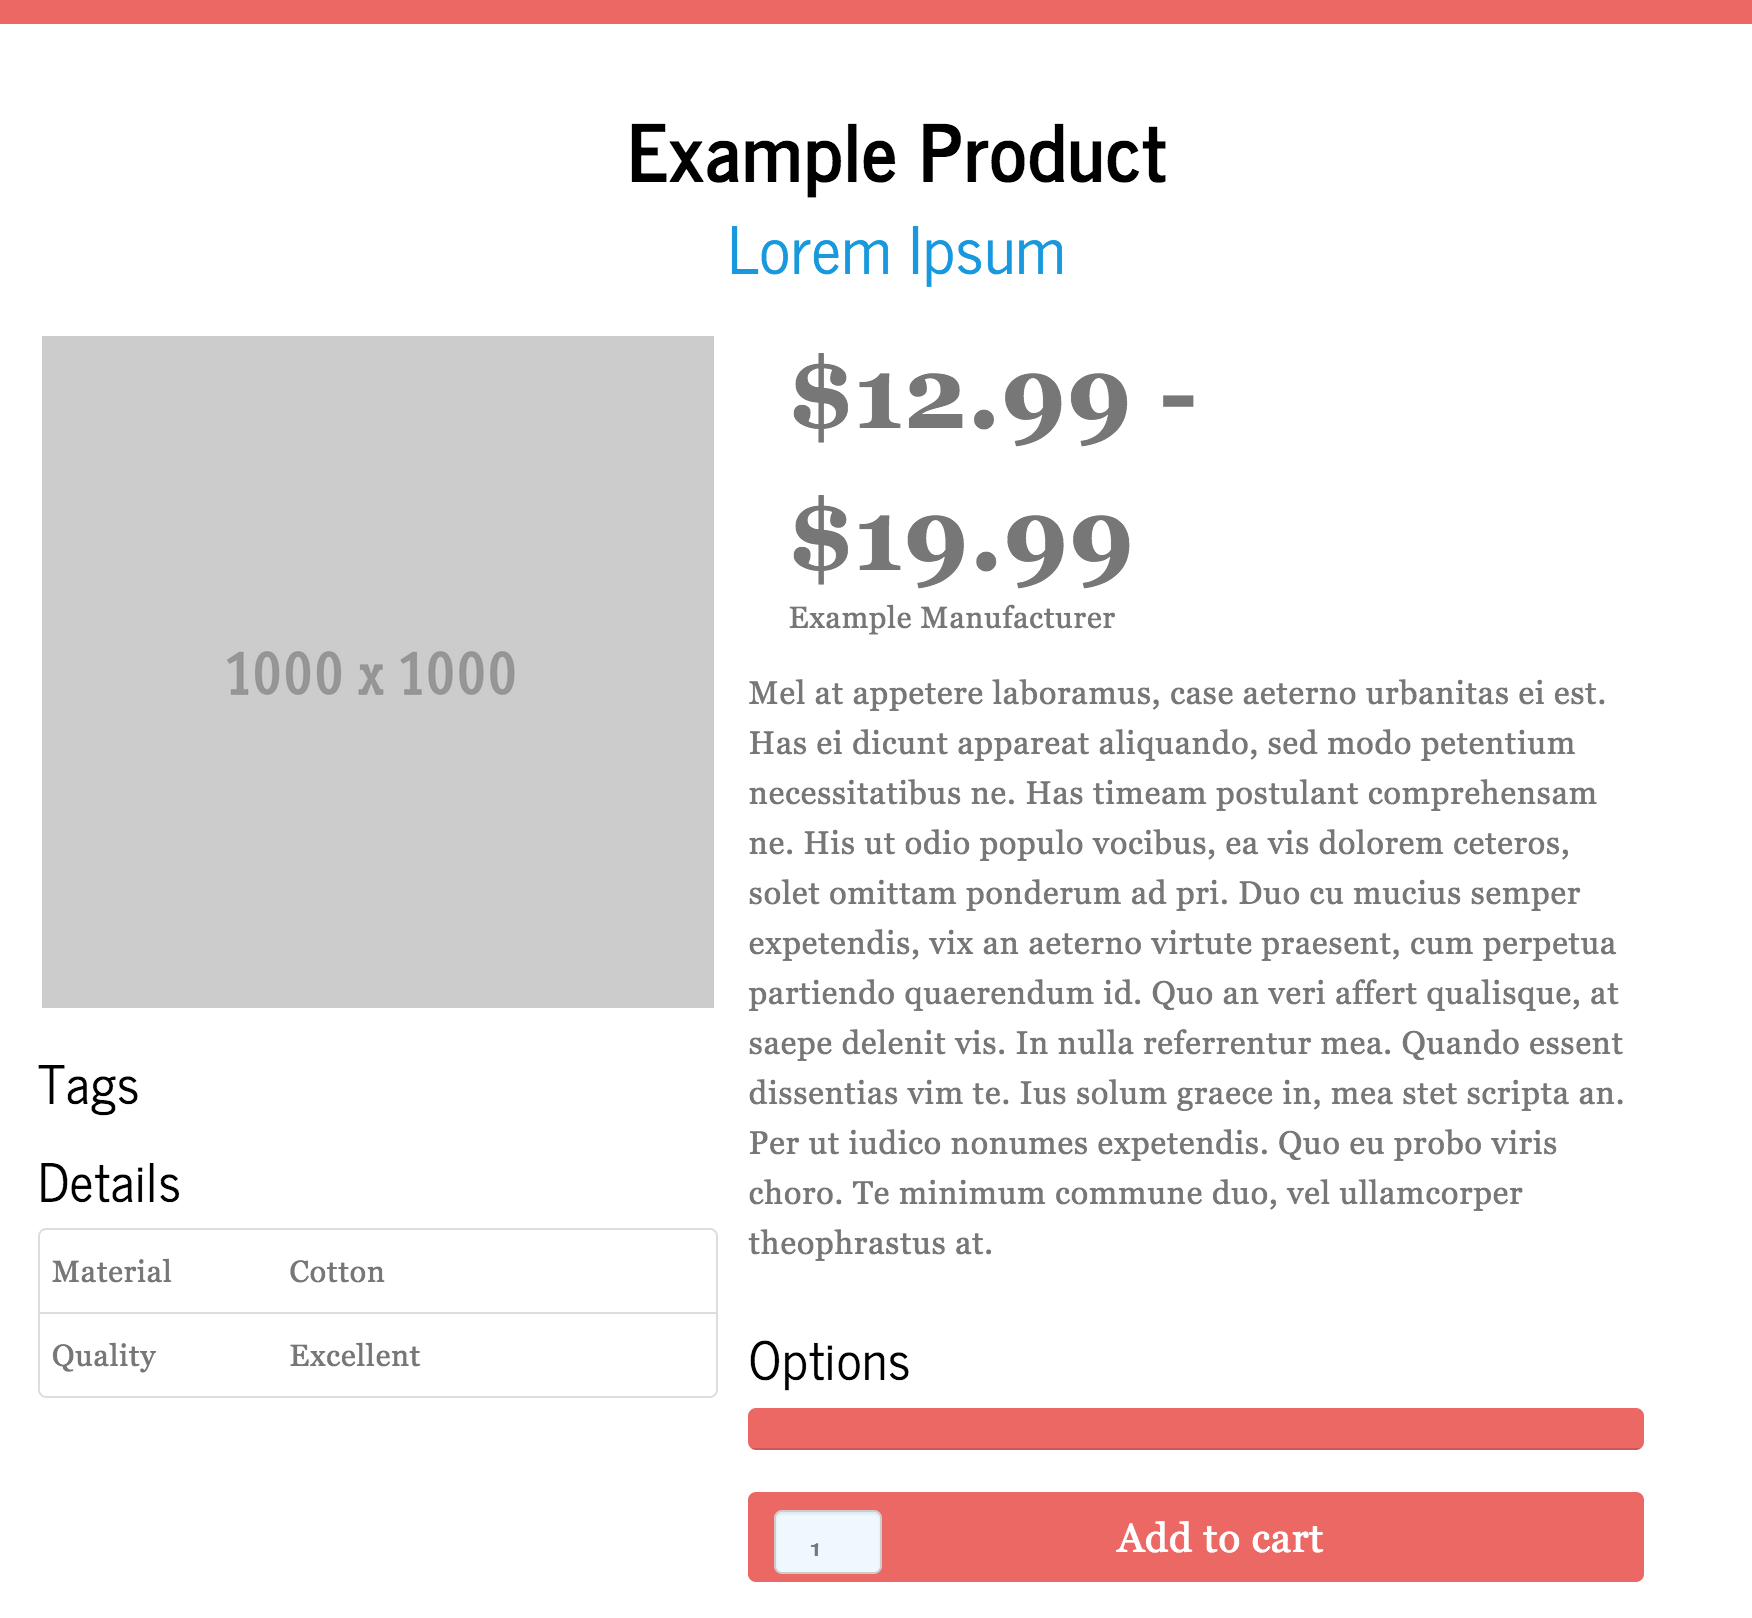
\includegraphics[width=0.6\textwidth]{figuras/bootstrap/bootstrap_theme_journal.png}

		\caption{Descripción de un producto utilizando el \themeCPT \textbf{\themeJournal} del sitio \bootswatchNAME.}
		\label{figure:bootstrap:theme_journal}
	\end{figure}

	\begin{figure}[H]
		\centering
		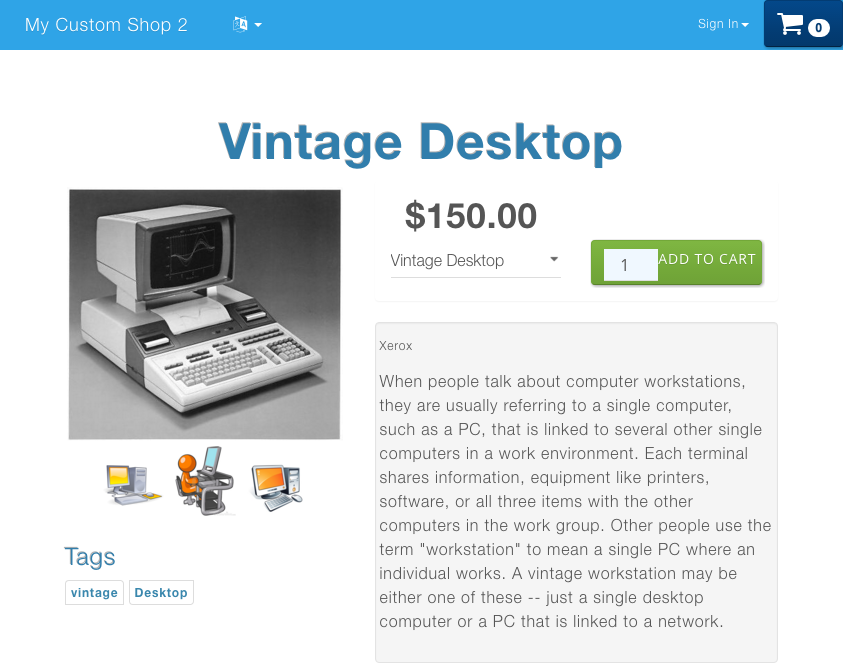
\includegraphics[width=0.6\textwidth]{figuras/bootstrap/bootstrap_theme_cerulean.png}

		\caption{Descripción de un producto utilizando el \themeCPT \textbf{\themeCerulean} del sitio \bootswatchNAME.}
		\label{figure:bootstrap:theme_cerulean}
	\end{figure}

	\begin{figure}[H]
		\centering
		\includegraphics[width=0.6\textwidth]{figuras/bootstrap/bootstrap_theme_superhero.png}

		\caption{Descripción de un producto utilizando el \themeCPT \textbf{\themeSuperHero} del sitio \bootswatchNAME.}
		\label{figure:bootstrap:theme_superhero}
	\end{figure}

	\begin{figure}[H]
		\centering
		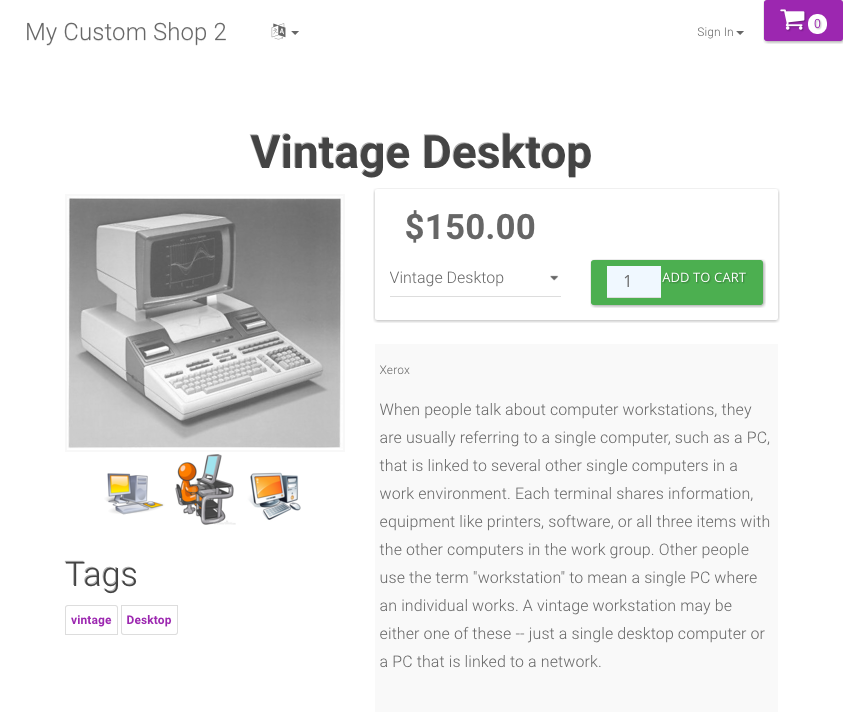
\includegraphics[width=0.6\textwidth]{figuras/bootstrap/bootstrap_theme_paper.png}

		\caption{Descripción de un producto utilizando el \themeCPT \textbf{\themePaper} del sitio \bootswatchNAME.}
		\label{figure:bootstrap:theme_paper}
	\end{figure}

	\begin{figure}[H]
		\centering
		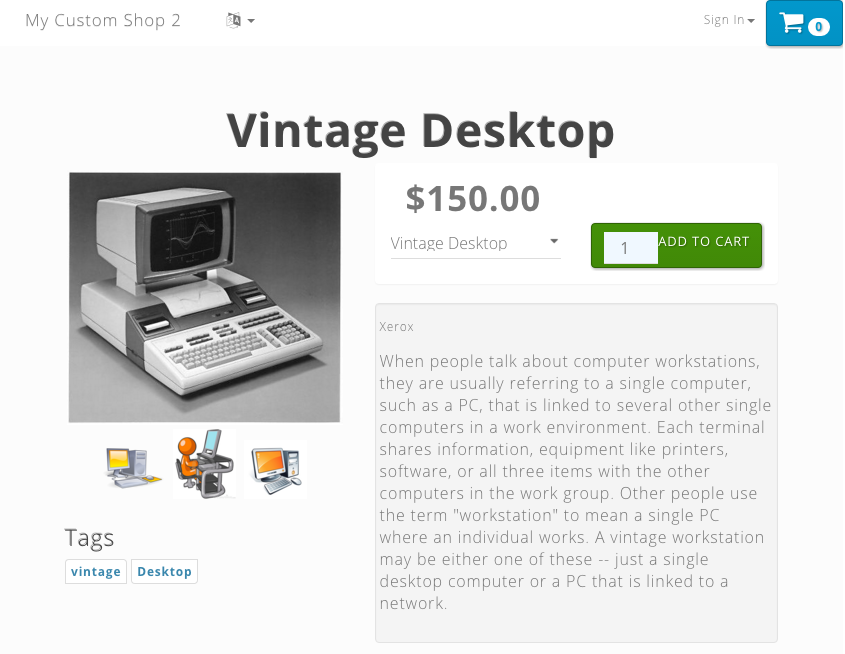
\includegraphics[width=0.6\textwidth]{figuras/bootstrap/bootstrap_theme_simplex.png}

		\caption{Descripción de un producto utilizando el \themeCPT \textbf{\themeSimplex} del sitio \bootswatchNAME.}
		\label{figure:bootstrap:theme_simplex}
	\end{figure}

	\begin{figure}[H]
		\centering
		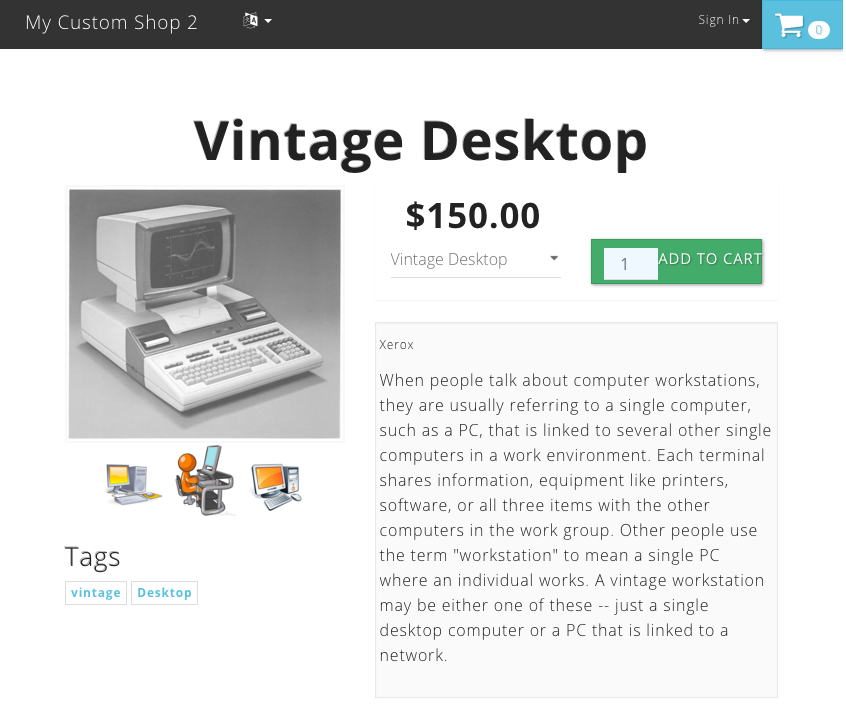
\includegraphics[width=0.6\textwidth]{figuras/bootstrap/bootstrap_theme_yeti.png}

		\caption{Descripción de un producto utilizando el \themeCPT \textbf{\themeYeti} del sitio \bootswatchNAME.}
		\label{figure:bootstrap:theme_yeti}
	\end{figure}